%%%%%%%%%%%%%%%%%%%%%%%%%%%%%%%%%%%%%%%%%
% UFPR Presentation
% LaTeX Template
% Version 1.0 (07/04/2016)
%
% Author: Vidal Daniel da Fontoura
% Site: http://www.inf.ufpr.br/vfontoura
%
%%%%%%%%%%%%%%%%%%%%%%%%%%%%%%%%%%%%%%%%%

%----------------------------------------------------------------------------------------
%	PACKAGES AND THEMES
%----------------------------------------------------------------------------------------

\documentclass{beamer} 

% The Beamer class comes with a number of default slide themes
% which change the colors and layouts of slides. Below this is a list
% of all the themes, uncomment each in turn to see what they look like.
% For more theme see http://www.hartwork.org/beamer-theme-matrix/

%\usetheme{default}
%\usetheme{AnnArbor}
%\usetheme{Antibes}
%\usetheme{Bergen}
%\usetheme{Berkeley}
%\usetheme{Berlin}
%\usetheme{Boadilla}
%\usetheme{CambridgeUS}
%\usetheme{Copenhagen}
%\usetheme{Darmstadt}
%\usetheme{Dresden}
\usetheme{Frankfurt}
%\usetheme{Goettingen}
%\usetheme{Hannover}
%\usetheme{Ilmenau}
%\usetheme{JuanLesPins}
%\usetheme{Luebeck}
%\usetheme{Madrid}
%\usetheme{Malmoe}
%\usetheme{Marburg}
%\usetheme{Montpellier}
%\usetheme{PaloAlto}
%\usetheme{Pittsburgh}
%\usetheme{Rochester}
%\usetheme{Singapore}
%\usetheme{Szeged}
%\usetheme{Warsaw}

% As well as themes, the Beamer class has a number of color themes
% for any slide theme. Uncomment each of these in turn to see how it
% changes the colors of your current slide theme.

%\usecolortheme{albatross}
%\usecolortheme{beaver}
%\usecolortheme{beetle}
%\usecolortheme{crane}
%\usecolortheme{dolphin}
%\usecolortheme{dove}
%\usecolortheme{fly}
%\usecolortheme{lily}
%\usecolortheme{orchid}
%\usecolortheme{rose}
%\usecolortheme{seagull}
\usecolortheme{seahorse}
%\usecolortheme{whale}
%\usecolortheme{wolverine}

\definecolor{light_green}{RGB}{230,255,230} % Create a background color
\definecolor{tbGreen}{RGB}{166,210,166}

\setbeamercolor{background canvas}{bg=light_green} % Apply the background color
%\useinnertheme{circles} %define os numeradores com o padrão circles
%\setbeamercolor{block title}{fg=white,bg=green!40!black} %define os titulos dos blocos como verde
%\setbeamercolor{itemize item}{fg=green!40!black} %define os marcadores de ítem como verdes
%\setbeamercolor{itemize subitem}{fg=green!40!black} %define os marcadores de sub-ítem como verdes
%\setbeamercolor{item projected}{fg=white,bg=green!40!black} %define os numeradores como verdes

\setbeamercolor{section in toc shaded}{fg=black} %define os links no tableofcontents como preto (quando estão selecionados)
\setbeamercolor{section in toc}{fg=black} %define os links no tableofcontents como preto (quando não estão selecionados)

\setbeamercolor{structure}{bg=black,fg=green!50!black}
%\setbeamercolor{title}{fg=black, bg=green!40!black}
%\setbeamercolor{frametitle}{fg=black, bg=green!80!black}


\setbeamertemplate{navigation symbols}{} % remover barra de navega‹o
%\setbeamertemplate{footline}[frame number] % numero de paginas

\setbeamertemplate{footline}
{
	\leavevmode%
	\hbox{%
		\begin{beamercolorbox}[wd=.333333\paperwidth,ht=2.25ex,dp=1ex,center]{author in head/foot}%
			\usebeamerfont{author in head/foot}\insertshortinstitute
		\end{beamercolorbox}%
	    \begin{beamercolorbox}[wd=.333333\paperwidth,ht=2.25ex,dp=1ex,center]{title in head/foot}%
			\usebeamerfont{title in head/foot}
		\end{beamercolorbox}%
		\begin{beamercolorbox}[wd=.333333\paperwidth,ht=2.25ex,dp=1ex,right]{date in head/foot}%
			\usebeamerfont{date in head/foot}\insertshortdate{}\hspace*{2em}
			\insertframenumber{} / \inserttotalframenumber\hspace*{2ex} 
		\end{beamercolorbox}
	}%
	\vskip0pt%
}

\usepackage[brazil]{babel} %Allow the use of brazilian portuguese language
%\usepackage[english]{babel}
%\usepackage[utf8x]{inputenc} % acento normal
\usepackage[utf8]{inputenc}

\usepackage{scalefnt}
\usepackage{color, colortbl, multirow}
\usepackage{epstopdf} % usar figura eps
\usepackage{verbatim} % para colocar o comment
\usepackage[portuguese,ruled,lined]{algorithm2e}
\usepackage{algorithmic}

\algsetup{linenosize=\tiny}

\setcounter{secnumdepth}{5}
\SetKwFor{Para}{para}{fa\c{c}a}{fim para}
\SetKwFor{ParaCada}{para cada}{fa\c{c}a}{fim para cada}
\SetKwBlock{Inicio}{inicio}{fim}

\usepackage{graphicx} % Allows including images
\usepackage{booktabs} % Allows the use of \toprule, \midrule and \bottomrule in tables

\usepackage{scalefnt}

\usepackage[export]{adjustbox}

\hypersetup{pdfpagemode=FullScreen}   % Full Screen
\hypersetup{pdfpagelayout=SinglePage} % Page layout

\pgfdeclareimage[height=0.5cm]{c-bio}{figuras/logo.png}
\pgfdeclareimage[height=0.5cm]{ufpr}{figuras/ufpr.png}
\logo{\pgfuseimage{ufpr} \hspace{320pt} \pgfuseimage{c-bio}}


%%===================== Capa =========================%%


\title[Short title]{\textbf{APLICANDO PROJETO AUTOMÁTICO DE HEURÍSTICAS
		DE ALTO NÍVEL NO PROBLEMA DE DOBRAMENTO DE
		PROTEÍNAS}} % The short title appears at the bottom of every slide, the full title is only on the title page

\author{Vidal Daniel da Fontoura} 
\institute[UFPR - Universidade Federal do Paraná] % Your institution as it will appear on the bottom of every slide, may be shorthand to save space
{
	Universidade Federal do Paraná \\ % Your institution for the title page
	Programa de Pós-Graduação em Informática
	
	Orientador(a): Prof.ª Dra Aurora Pozo \\
	Co-Orientador(a): Prof. Dr Roberto Santana 
}

\date{\today} % Date, can be changed to a custom date. You can use \day \month \year or \today, for example.

\begin{document} % inicio do documento

\frame{
	\titlepage
}

%%===========================ROTEIRO=============================%%
\begin{frame}{Agenda}	


   \hspace*{1cm}
	%\begin{minipage}[t][6cm][t]{\textwidth}
		\vspace{-30pt}
		\tableofcontents
	%\end{minipage}
\end{frame}

%%========================Introducao================================%%
\section{Introdução}

%%========================Objetivo================================%%








\subsection{Checkar oque por aqui}
\frame{
	\frametitle{Checkar oque por aqui}
	
	\begin{block}{Checkar oque por aqui}
	
	\end{block}
}








%%========================Introducao================================%%
\section{Dobramento de Proteínas}

%%========================Objetivo================================%%
\subsection{Proteínas}
\frame{
	\frametitle{Proteínas}

		\begin{itemize}
			\item 	Estruturas compostas por uma ou mais cadeias de aminoácidos.
			\item 	Exercem um papel fundamental na natureza.
			\item   Responsáveis por muitas funções importantes da células vivas.
			\item 	São produtos de um processo chamado dobramento de proteínas.
			\item	Inicia a partir de uma cadeia de aminoácidos inicialmente desdobrada que será transformada em sua estrutura final/nativa.
		\end{itemize}

}

\subsection{Problema de Dobramento Proteínas}
\frame{
	\frametitle{Problema de Dobramento de Proteínas}
		\begin{itemize}
			\item Preocupa-se em entender o processo de dobramento das proteínas.
			\item Também trata da predição das estruturas de proteínas.
			\item A predição das estruturas tem um amplo campo de aplicações:
			\begin{itemize}
				\item Síntese de novas proteínas e dobramentos.
				\item Síntese de novas drogas baseada nas estruturas.
				\item Obtenção de estruturas a partir de dados
				incompletos de ressonância magnética nuclear.
			\end{itemize}
			\item A determinação da estrutura nativa de proteínas é uma tarefa desafiadora até mesmo para modernos super computadores.
			\item Trata-se de um problema $NP$-Completo.
		\end{itemize}
}

\frame{
	\frametitle{Modelos de Representação de Proteínas}
		\begin{itemize}
			\item Diferentes modelos para representar proteínas existem.
			\item Modelos extremamente detalhados são computacionalmente caros.
			\item Modelos simplificados são largamente utilizados por pesquisadores por conta de sua simplicidade em representar as proteínas.
			\item Modelo Hidrofóbico-Polar (HP).
		\end{itemize}

}


\begin{frame}[allowframebreaks]{Modelo Hidrofóbico-Polar}
	

		\begin{itemize}
			\item Generaliza os aminoácidos que compõem as proteínas em apenas dois aminoácidos: hidrofóbicos H ou polares P.
			\item Utiliza um \textit{grid} 2d ou um cubo 3d para representar as possíveis conformações de uma proteína.
			\item No modelo HP existem 3 interações entre os aminoácidos H-P, P-P e H-H.
			\item Para calcular a energia de uma conformação no modelo HP é necessário avaliar a quantidade de interações hidrofóbicas (H-H) entre aminoácidos não consecutivos na sequência.
		\end{itemize}
		
		\begin{figure}[!htb]
			\centering
			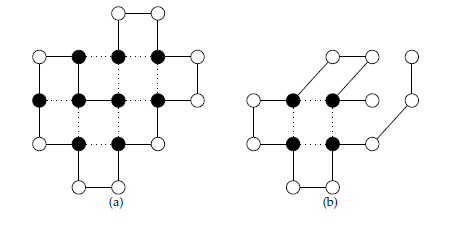
\includegraphics[scale=.8]{figuras/modeloHPExemplo.png}
			\caption{Exemplos de representação de proteínas utilizando os modelos HP 2D-HP (a) e 3D-HP (b). Fonte: Adaptado de \cite{santanna2008} }
			\label{fig:exemploModeloHP}
		\end{figure}

\end{frame}



\begin{frame}[allowframebreaks]{Representação do Problema}
	
	\begin{itemize}
		\item Existem várias maneiras de representar as conformações no modelo HP.
		\item 	Coordenadas relativas: O conjunto de movimentos possíveis para a grade 2D é definido por $\{F,E,D\}$, que correspondem aos movimentos: frente (continuar no mesmo sentido do aminoácido anterior), à esquerda e à direita. 
		\item Geralmente se utiliza uma codificação utilizando números inteiros, como por exemplo:  F$->$0, E$->$1 e D$->$2. 
	\end{itemize}
	
	\begin{figure}[!htb]
		\centering
		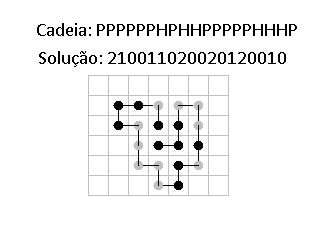
\includegraphics[scale=.8]{figuras/ExemploCodificacao.png}
		\caption{Exemplo de conformação gerada por uma solução codificada utilizando coordenadas relativas para uma cadeia de 20 aminoácidos.  Fonte: Autoria Própria }
		\label{fig:exemploCodificacao}
	\end{figure}



	
\end{frame}

	

%%========================Introducao================================%%
\section{Hiper-Heurísticas}

%%========================Objetivo================================%%
\frame{
	\frametitle{Hiper-Heurísticas}
	

		\begin{itemize}
			\item   Ainda existem dificuldades de generalização de métodos heurísticos. 
			\item  Esta dificuldade surge  da necessidade de selecionar
			os parâmetros e configurações mais adequados dos algoritmos para um problema ou instância.
			\item  Questão: \textbf{É possível
			automatizar o projeto e parametrização de métodos heurísticos para resolver problemas
			de busca computacional difíceis?}
			\item A ideia principal é desenvolver algoritmos que sejam
			mais genéricos do que as implementações de metodologias atuais.
		\end{itemize}
		
		

}


\frame{
	\frametitle{Hiper-Heurísticas}
	

		\begin{itemize}
		\item Operam sobre o
		espaço de busca de heurísticas que operam sobre o espaço de busca  de um determinado problema.
		\item O objetivo
		principal é tentar selecionar ou gerar a heurística mais adequada para cada situação.
		
		\item Geralmente \textit{frameworks} hiper-heurísticos possuem dois níveis: Alto e Baixo.
		\end{itemize}
}

\frame{
	\frametitle{Hiper-Heurísticas}
		\begin{itemize}
	\item \textbf{Heurísticas de alto nível}: Geralmente consistem em dois componentes: \textbf{mecanismo
	de seleção} e um \textbf{critério de aceitação}.
	\item \textbf{Heurísticas de baixo nível}:  Um conjunto de heurísticas de baixo nível específicas. São exemplos: \textbf{operadores
	de cruzamento, mutação e buscas locais}. Em alguns casos, \textbf{meta-heurísticas} também  assumem o papel de
	heurísticas de baixo nível.
			\end{itemize}

}


\frame{
	\frametitle{\textit{Framework} Geral Hiper-Heurísticas}

		\begin{figure}[!htb]
			\centering
			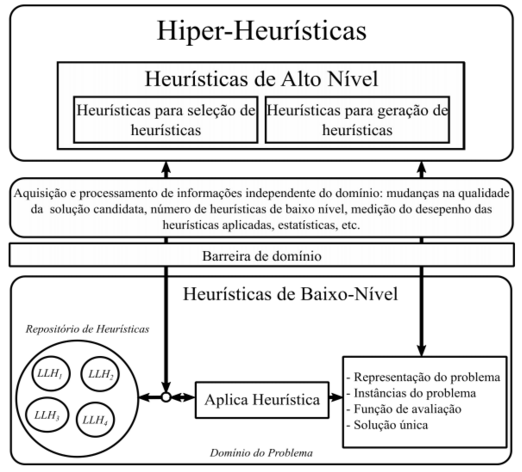
\includegraphics[scale=.6]{figuras/HiperHeuristicas.png}
			\caption{\textit{Framework} Geral Hiper-Heurístico. Adaptado de \cite{sabar2015automatic}}
			\label{img:hiperheuristico}
		\end{figure}

}

%\frame{
%	\frametitle{Classificação Hiper Heurísticas}
%	
%
%		\begin{figure}[!htb]
%			\centering
%			\includegraphics[scale=.5]{figuras/ClassificacaoHiperHeuristica.png}
%			\caption{Classificação Hiper Heurísticas}
%			\label{fig:classificacaoHH}
%		\end{figure}
%
%}


\subsection{Hiper-Heurísticas de Seleção}
\frame{
	\frametitle{Hiper-Heurísticas de Seleção}
	

		\begin{itemize}
			\item \textbf{Random} (R):  Seleciona aleatoriamente as heurísticas a serem aplicadas.
			\item \textbf{Choice Function} (CF):  Função que leva em consideração o desempenho das heurísticas assim como quanto tempo se passou desde a última execução de uma heurística \cite{burke2013hyper}.
			\item \textbf{Greedy} (GR): Realiza as escolhas de maneira gulosa levando em consideração o desempenho das heurísticas \cite{burke2013hyper}.
			\item \textbf{Tabu Search Based} (TS): Utiliza uma lista tabu para evitar determinadas heurísticas que não apresentaram bom desempenho \cite{burke2013hyper}.
			\item \textbf{Multi-Armed Bandit} (MAB): Utiliza uma função baseada em dois componentes: um referente à qualidade e  um intervalo de confiança baseado no número de vezes que a heurística foi aplicada \cite{burke2013hyper}.
		\end{itemize}

}



\frame{
	\frametitle{Critérios de Aceitação}

			\begin{itemize}
				\item \textbf{All Moves} (AM): Aceita qualquer aplicação de heurísticas mesmo que seja sem melhora na solução \cite{burke2013hyper}.
				\item \textbf{Improvemnt Only} (IO): Aceita apenas aplicações de heurística que melhoraram uma solução \cite{burke2013hyper}.
				\item \textbf{Monte Carlo} (MC): Aceita aplicações de heurísticas que melhoram uma solução e utiliza probabilidades para aceitar aplicações que não melhoram \cite{burke2013hyper}.
				\item \textbf{Great Deluge} (GD): Esta estratégia estende o algoritmo \textit{Great Deluge} para decidir quando aceitar soluções geradas pelas heurísticas \cite{burke2013hyper}.				
			\end{itemize}
}



\section{Programação Genética (PG)}
\frame{
	\frametitle{Programação Genética (PG)}
		\begin{itemize}
			\item É um ramo da síntese de programas que utiliza ideias oriundas
			da teoria da evolução natural para produzir programas.
			\item Uma população aleatória de programas de computador é gerada, e os
			operadores geneticamente inspirados (cruzamento e mutação) são repetidamente aplicados
			com objetivo de produzir novos programas de computador.
			
			\item Estes programas são avaliados
			utilizando uma função de \textit{fitness} que determina quais destes programas são mais
			suscetíveis a sobreviver para gerações futuras.
			\item Os programas
			que compõem a população são representados utilizando estruturas de árvore.
			\item Outras estruturas podem ser evoluídas.
		\end{itemize}

}


\subsection{Evolução Gramatical (EG)}
\frame{
	\frametitle{Evolução Gramatical (EG)}
	

		
		\begin{itemize}
		\item Técnica relativamente nova de computação evolutiva, proposta por Ryan et al. \cite{ryan1998grammatical}, trata-se de um tipo de programação genética. 
		\item Objetivo é encontrar um programa executável ou trecho
		de um programa, que obtenha um bom valor de \textit{fitness} para o problema em questão.
		\item Utiliza vetores de inteiros para representar seus indivíduos e uma gramática BNF específica para traduzir os indivíduos em programas de computador.
		\item Uma gramática BNF possui um 
		conjunto de terminais e não terminais, que podem ser expandidos em um ou mais terminais e
		não terminais.
		\end{itemize}

}

\frame{
	\frametitle{Gramática Exemplo}
	

			\begin{figure}[!htb]
				\centering
				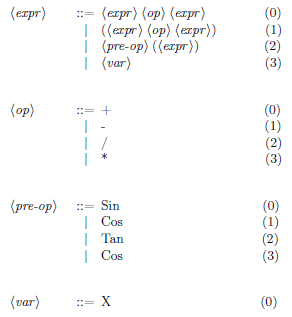
\includegraphics[scale=.8]{figuras/GramaticaExemplo.png}
				\caption{Gramática Exemplo}
				\label{fig:gramaticaExemplo}
			\end{figure}
	

}

\frame{
	\frametitle{Exemplo de decodificação de cromossomo}
	


		[valor do vetor] mod [quantidade de opcoes] = indice da opcao
		

		Vetor exemplo: 24 27 10 14 12 23 16 20
	
		\begin{itemize}
					\item 24 mod 4 = 0  $\to  \langle expr \rangle$  $\langle op \rangle$  $\langle expr \rangle$ 
					\item 27    mod 4 = 3  $\to  \langle var\rangle$  $\langle op\rangle$  $\langle expr\rangle \to   X \langle op\rangle  \langle expr\rangle$ 
					
					\item 10  mod 4 = 2 $ \to X / \langle expr\rangle$
					
					
					\item 14  mod 4 = 2  $ \to  X / (\langle pre-op\rangle  \langle expr\rangle)$  
					
					\item 12 	mod 4 = 0 $ \to  X / (Sin \langle expr\rangle )$
					
					
					\item 23 	mod 4 = 3 $ \to X / (Sin \langle var\rangle ) \to X / (Sin X)$
					

			
		\end{itemize}
							Expressão final: $X / (Sin X)$
	
}


%\frame{
%	\frametitle{Operadores para evolução gramatical}
%	
%
%			 Além dos operadores tradicionais outros dois operadores \textit{Prune} e \textit{Duplicate} são peculiares à EG e serão descritos em seguida:
%			 
%			 \begin{itemize}
%			 	\item \textbf{Duplicate}: Dada uma probabilidade realiza a cópia de alguns genes ao final do indivíduo. O número de genes a serem duplicados é selecionado de maneira aleatória. A motivação por trás deste operador é que ao duplicar genes ocorre um aumento da presença de genes que são potencialmente bons, pois pertencem a um indivíduo com boa aptidão selecionado pelo operador de seleção.
%			 	\item \textbf{Prune}: Leva em consideração que nem sempre todos os genes, de um cromossomo, são utilizados para decodificar um programa. Dessa maneira (dada uma probabilidade) realiza o truncamento de  cromossomos. O objetivo é diminuir a probabilidade que o operador de cruzamento opere em regiões dos cromossomos que não sejam utilizadas realmente.
%			 \end{itemize}
%}


\frame{
	\frametitle{Pseudocódigo da evolução gramatical}
	
	

				\begin{figure}[!htb]
					\centering
					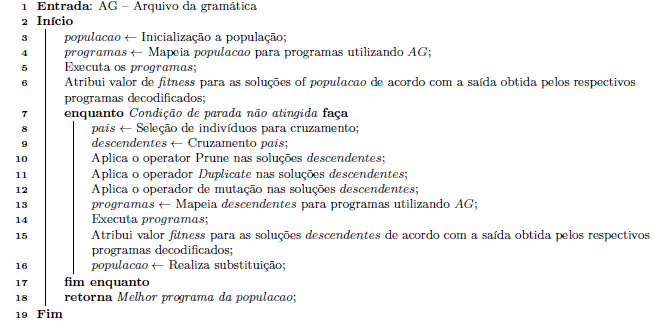
\includegraphics[scale=.6]{figuras/PseudocodigoEG.png}
					\caption{Pseudocódigo da evolução gramatical.}
					\label{fig:pseudocodigoEG}
				\end{figure}
				


}



%%===================Método proposto==============%%
\section{Método Proposto}
\subsection{Método Proposto}
\frame{
  \frametitle{Método Proposto}
   

      	\begin{itemize}
      	 \item Esta proposta visa a aplicação da EG para geração de heurísticas
      	 de alto nível para uma plataforma hiper-heurística para o PDP (HyPDP).
      	 \item Baseada no trabalho desenvolvido por Sabar et al. \cite{sabar2015automatic}.
      	 \item No contexto desta proposta:
      	   \begin{itemize}
	      	 \item Heurísticas de alto nível consistem de um \textbf{mecanismo de seleção} e um \textbf{critério de aceitação}. 
	      	 \item Heurísticas de baixo nível são compostas por um conjunto de heurísticas, selecionadas de
	      	 estudos anteriores, um mecanismo de memória e uma função de \textit{fitness}.
      	   \end{itemize}
      	\end{itemize}

}

\frame{
	\frametitle{Método Proposto}

		\begin{figure}[!htb]
			\centering
			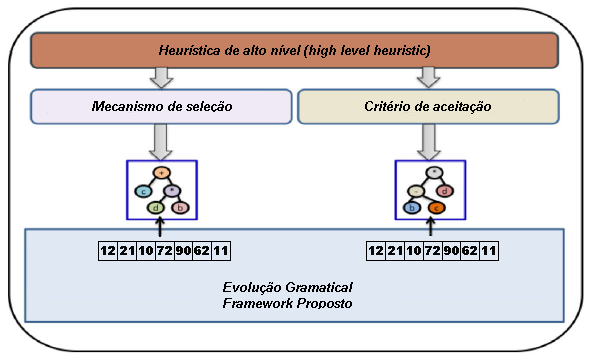
\includegraphics[scale=.8]{figuras/ProposedFramework.png}
			\caption{Método proposto}
			\label{fig:proposedFramework}
		\end{figure}	

}



\subsection{Gramática Proposta}
\frame{
	\frametitle{Gramática Proposta}

		\begin{figure}[!htb]
			\centering
			
\includegraphics[scale=.6]{figuras/ProposedGramatica.png}
			\caption{Gramática para converter vetores de inteiros em heurísticas de alto nível.}
			\label{fig:proposedGrammar}
		\end{figure}
		

}


\subsection{Terminais para gerar mecanismos de seleção}
\frame{
	\frametitle{Terminais para gerar mecanismos de seleção}
	

		\begin{itemize}
			\item RC (\textit{Reward Credit}): Recompensa que uma determinada heurística de baixo nível deve receber baseado no seu desempenho. O cálculo da melhoria é dado por: $M(i) = (|f1 -f2|/f1) *100$ se $f2 < f1$, onde $f1$ é a qualidade da solução corrente e $f2$ é a qualidade da solução resultante. 
			A melhoria obtida é salva em uma janela deslizante (FIFO) de tamanho W. O crédito de qualquer heurística de baixo nível é então atribuído como o máximo valor na janela deslizante correspondente. 
			%A ideia por trás deste critério é: heurísticas de baixo nível que não são usadas com frequência mas que alteram a solução com grandes melhorias tendem a ter mais preferência do que aquelas que geram pequenas melhorias. Portanto as heurísticas que trazem frequentes, mas pequenas melhorias irão ter menos probabilidade de serem selecionadas.
			\item \textbf{$C_{best}$}: Número de vezes que a i-ésima heurística de baixo nível atualizou a melhor solução conhecida. Este critério favorece as heurísticas de baixo nível que obtiveram êxito em melhorar a melhor solução conhecida até o momento. Este critério é útil para sistematicamente melhorar o atual mínimo local.
		  
		\end{itemize} 
		
		

}


\subsection{Terminais para gerar mecanismos de seleção (cont.)}
\frame{
	\frametitle{Terminais para gerar mecanismos de seleção (cont.)}
	

		\begin{itemize}
			\item $C_{current}$: Número de vezes que a i-ésima heurística de baixo nível atualizou a solução atual. Este critério favorece as heurísticas de baixo nível que obtém êxito em atualizar a solução corrente. Este critério serve para deixar a busca concentrada próxima à solução corrente.
			\item $C_{accept}$: Número de vezes que a solução gerada pela i-ésima heurística de baixo nível foi aceita pelo critério de aceitação. Irá favorecer heurísticas de baixo nível que podem ajudar a escapar de um mínimo local.
			\item $C_{ava}$: A média de melhorias anteriores da i-ésima heurística de baixo nível. Este critério favorece heurísticas de baixo nível que realizaram grandes melhorias em média.
			\item $C_r$: O número de vezes que a i-ésima heurística de baixo nível foi classificada como primeira.
			
		\end{itemize} 
			

}


\subsection{Terminais para gerar critérios de aceitação}
\frame{
	\frametitle{Terminais para gerar critérios de aceitação}

	 \begin{itemize}
		 	\item Delta: A diferença da qualidade entre a solução corrente e a solução descendente.
		 	\item PF: A qualidade da solução anterior.
		 	\item CF: A qualidade da solução atual.
		 	\item CI: Iteração corrente.
		 	\item TI: Número de iterações.
	 \end{itemize}
		
		

}



\subsection{Funções matemáticas para gerar as heurísticas de alto nível}
\frame{
	\frametitle{Funções matemáticas para gerar as heurísticas de alto nível}

		 \begin{itemize}
		 	\item +: Adiciona as duas entradas.
		 	\item -: Subtrai a segunda entrada da primeira.
		 	\item *: Multiplica as duas entradas.
		 	\item \%: Divisão protegida, isto é, se o denominador for 0, o altera para 0,001.
		 \end{itemize}

}


\subsection{EG para gerar heurísticas de alto nível}
\frame{
	\frametitle{Método Proposto}
	

		\begin{itemize}
			\item Utilizando a gramática apresentada e vetores de inteiros é possível gerar heurísticas de alto
			nível. Os conjuntos terminais da gramática apresentam estatísticas sobre as heurísticas de
			baixo nível e estas são a matéria-prima para a construção dos componentes das heurísticas
			de alto nível para o HyPDP.
			
			\item O próximo passo consiste em evoluir uma população de vetores de inteiro, gerados de
			maneira aleatória, utilizando o processo evolutivo descrito anteriormente.
		\end{itemize}
		
		

}


\subsection{Função de fitness para a evolução gramatical}
\frame{
	\frametitle{Função de \textit{fitness} para a evolução gramatical}
	
			\begin{itemize}
			\item Uma função de \textit{fitness} baseada na função proposta por Sabar et al. \cite{sabar2015automatic} foi desenvolvida para esta proposta.
			
			\item A probabilidade de selecionar indivíduos é alterada de acordo com a qualidade
			da melhor solução retornada pela execução da plataforma  hiper-heurística HyPDP, utilizando
			o mecanismo de seleção e critério de aceitação.
			
			\item A
			qualidade retornada pela solução pode ser pior ou melhor do que a solução utilizada como
			entrada para a plataforma hiper-heurística.
		
			\end{itemize}
		
}


\subsection{Função de fitness para a evolução gramatical}
\frame{
	\frametitle{Função de \textit{fitness} para a evolução gramatical}		

Suponha que $f_i$ e $f_b$ representem a qualidade da solução inicial e da retornada e $Ph[]$ o vetor de probabilidades de seleção dos indivíduos da EG. A retribuição para o $i-$ésimo indivíduo, caso tenha obtido uma melhoria, é calculada utilizando a equação \ref{eq:fitnessFunction1}.

	\begin{block}{Função de \textit{fitness} para retribuição ao $i-$ésimo indivíduo}
		
		 \begin{equation} {}
		 \label{eq:fitnessFunction1}
		 Ph[i] = Ph[i] + \sigma 
		 \end{equation}
		  Onde:
		 \begin{equation}
					 \sigma = (f_i - f_b)/(f_i + f_b). 
		 \end{equation}		
	\end{block}
}





\subsection{Função de fitness para a evolução gramatical}
\frame{
	\frametitle{Função de \textit{fitness} para a evolução gramatical}		
	
	Os demais indivíduos diferente de $i$ devem receber uma penalização. Suponha que $Nh$ seja o número de indivíduos a penalização é calculada utilizando a equação \ref{eq:fitnessPenalizeFunction1}.
	\begin{block}{Função de \textit{fitness} para penalização aos outros indivíduos $j$}
		\begin{equation} {}
		\label{eq:fitnessPenalizeFunction1}
		Ph[j] = Ph[j] - (\sigma / (Nh - 1))
		\end{equation}
		Tal que:	
		\begin{equation} {}
		\label{eq:fitnessPenalizeFunction2}
		j \in \{1, ..., Nh\} ~e~ j \neq i
		\end{equation}
		
	\end{block}
}	


\subsection{Função de fitness para a evolução gramatical}
\frame{
	\frametitle{Função de \textit{fitness} para a evolução gramatical}		
	
	Caso contrário (se a solução retornada não for melhor que a utilizada como entrada), uma penalização é aplicada ao $i$-ésimo indivíduo utilizando a equação \autoref{eq:fitnessBadFunction1}.
	\begin{block}{Função de \textit{fitness} para penalização do $i-$ésimo indivíduo}
		\begin{equation} {}
		\label{eq:fitnessBadFunction1}
		Ph[i] = Ph[i] - |\sigma \times \alpha|
		\end{equation}
		
		Onde: 
		\begin{center}
			$\alpha =$ iteração corrente $/$ número total de iterações.
		\end{center} 
	\end{block}	
}


\subsection{Função de fitness para a evolução gramatical}
\frame{
	\frametitle{Função de fitness para a evolução gramatical}		
	
	Os demais indivíduos $j \neq i$ recebem uma recompensa utilizando a \autoref{eq:fitnessOtherFunction} 

	\begin{block}{Função de \textit{fitness} para retribuição dos outros indivíduos $j$}
		\begin{equation} {}
		\label{eq:fitnessOtherFunction}
		 Ph[j] = Ph[j] + (|\sigma| \times \alpha / (Nh -1))
		\end{equation}
		
		 Tal que: 
		\begin{center}
		 $j \in \{1, ..., Nh\} ~e~ j \neq i$
		\end{center} 
		
		Onde:
		\begin{center}
		$Nh$ = número de indivíduos da EG \\ $\alpha =$ iteração corrente $/$ número total de iterações \\
		 $\sigma = (f_i - f_b)/(f_i + f_b)$
			
			
		\end{center}
	\end{block}	
}	

\subsection{Conjunto de heurísticas de baixo nível}
\frame{
	\frametitle{Conjunto de heurísticas de baixo nível}		
	\begin{itemize}
		\item \textit{Two Points Crossover} (2X): 
		
		\begin{figure}[!htb]
			\centering
			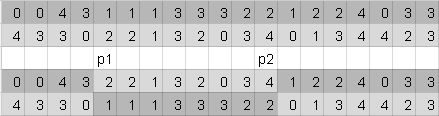
\includegraphics[scale=0.7]{figuras/TwoPointsCrossover.png}
			\caption{Exemplo de aplicação do operador 2x. Fonte Autoria Própria}
			\label{fig:twopointscrossover}
		\end{figure}
		
		
		\item \textit{Multi Points Crossover} (MPX): 
		
		\begin{figure}[!htb]
			\centering
			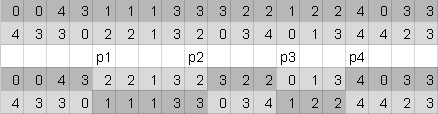
\includegraphics[scale=0.7]{figuras/MultiPointsCrossover.png}
			\caption{Exemplo de aplicação do operador MPX. Fonte Autoria Própria}
			\label{fig:multipointscrossover}
		\end{figure}
		
		
	\end{itemize} 
	
	
}



\frame{
	\frametitle{Conjunto de heurísticas de baixo nível}		
	\begin{itemize}
		
		
	
		\item \textit{Segment Mutation} (SMUT): Altera um número aleatório (5 a 7) de genes consecutivos para direções distintas. 
		
		\begin{figure}[!htb]
			\centering
			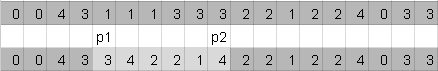
\includegraphics[scale=0.8]{figuras/segmentMutation.png}
			\caption{Exemplo de aplicação do operador SMUT. Fonte Autoria Própria}
			\label{fig:segmentMutation}
		\end{figure}
		
		
		\item \textit {Exhaustive Search Mutation} (EMUT): Esta heurística seleciona um gene aleatório e testa todas as outras direções possíveis e irá manter a alteração que conseguir aumentar a qualidade da conformação.
		
	\end{itemize} 
	
}


\frame{
	\frametitle{Conjunto de heurísticas de baixo nível}		
	\begin{itemize}
		
		
		
	\item \textit{Local Move Operator} (LM): Esta heurística troca direções entre dois genes aleatórios consecutivos.
	
	
	\begin{figure}[!htb]
		\centering
		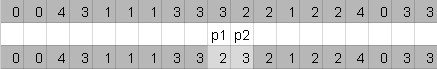
\includegraphics[scale=0.8]{figuras/LocalMoveOperator.png}
		\caption{Exemplo de aplicação do operador LM. Fonte Autoria Própria}
		\label{fig:localMoveOperator}
	\end{figure}
		
		
	\item \textit{Loop Move Operator} (LPM): Esta heurística troca direções entre dois genes que estão a 5 genes de distância na sequência, criando um movimento de \textit{loop}.
	
	
	\begin{figure}[!htb]
		\centering
		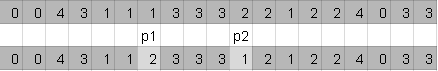
\includegraphics[scale=0.8]{figuras/LoopMoveOperator.png}
		\caption{Exemplo de aplicação do operador LPM. Fonte Autoria Própria}
		\label{fig:loopMoveOperator}
	\end{figure}	
	\end{itemize} 
	
}




\begin{frame}[allowframebreaks]{Processo geral da EG proposta}	
	
	\begin{itemize}
		\item Gerar população inicial de maneira aleatória e calcular o \textit{fitness} dos indivíduos inserindo-os no HyPDP e executando por um determinado número de iterações.
		\item De maneira iterativa selecionar indivíduos pais e aplicar os operadores
		de cruzamento, \textit{prune}, mutação, e \textit{duplicate} para gerar descendentes. Para avaliar os descendentes, os seguintes passos serão executados:
		\begin{itemize}
			\item Decodificar os indivíduos em heurísticas de alto nível.
			\item Executar o mecanismo de seleção com objetivo de ordenar as heurísticas de baixo nível.
			\item Selecionar de maneira aleatória uma solução do mecanismo de memória. Aplicar a heurística de baixo nível classificada com maior valor e calcular a qualidade da solução gerada.
			\item Se a solução gerada tiver qualidade superior à atual, a atual é substituída. Caso contrário a expressão referente ao critério de aceitação será executada.A  solução gerada pela
			heurística de baixo nível é aceita caso o exponencial natural do valor, retornado pelo
			critério de aceitação, seja menor ou igual a 0.5
			\item Aplicar a heurística de baixo nível, que foi selecionada pelo mecanismo de seleção,
			repetidamente até que não ocorram mais melhorias.
			\item Se não houverem mais melhorias, troca-se a heurística de baixo nível atual pela
			segunda melhor classificada, baseando-se no valor retornado pelo mecanismo de
			seleção.
			\item Se a etapa anterior chegar fim da lista de heurísticas de baixo nível, é executado o
			mecanismo de seleção novamente e a lista de heurísticas de baixo nível é reordenada.
			A busca reinicia agora utilizando a heurística de baixo nível com maior valor para
			a expressão referente ao mecanismo de seleção.
			\item O HyPDP continuará utilizando as heurísticas de alto
			nível por um tempo pré-determinado
			de iterações.
			\item A solução gerada ao final da busca será avaliada para
			entrar ou não no mecanismo de memória.
		\end{itemize}
		\item O processo da EG só irá terminar quando o critério de parada for atingido e será retornado o indivíduo (heurística de alto nível) que possuir o maior \textit{fitness}. Também será retornada a solução do mecanismo de memória que tiver a maior qualidade.
	\end{itemize}

\end{frame}



\begin{frame}[allowframebreaks]{Mecanismo de Memória}	
	
	\begin{itemize}
		\item Baseado no trabalho de Sabar et al. \cite{sabar2015automatic} um mecanismo de memória será desenvolvido para o HyPDP para armazenar soluções de alta qualidade e diversificadas entre si.
		\item A inicialização do mecanismo de memória será feita parte de maneira aleatória e parte utilizando uma estratégia de \textit{backtracking} para garantir que soluções válidas sejam geradas.
		\item A atualização do mecanismo de memória irá ocorrer toda vez que o HyPDP terminar a busca. 
		\item Para uma solução entrar no mecanismo de memória sua qualidade e sua diversidade irão ser avaliadas: a qualidade da solução é dada pela quantidade de iterações H-H multiplicada por -1.
		\item  As soluções geradas que tiverem a qualidade maior que todas as soluções contidas no mecanismo de memória substituirão a solução que tiver menor similaridade segundo a distância de \textit{Hamming} \cite{hamming1950error}.
		\item Se a qualidade de uma solução gerada não for maior que todas as soluções, mas melhor em relação a um sub-conjunto do mecanismo de memória, esta substituirá a solução que tiver menor qualidade e menor similaridade do sub-conjunto.
		\item E
		por fim se a qualidade da solução gerada for pior que todas contidas no mecanismo de
		memória, esta é descartada
		
			
	\end{itemize}
	
\end{frame}



\begin{frame}[allowframebreaks]{Avaliação da Abordagem Proposta}	
	

		
		\begin{table}[!htb]
			\scalefont{0.5}
			\begin{center}		
				\label{tab:sequences}
				{$\begin{array}{c r r l}
					\text{Id} & \text{Tamanho} &  \multicolumn{1}{c}{\text{Valor ótimo}} & \multicolumn{1}{c}{\text{Sequência}} \\ \hline
					s1 &20 &-9 & HPHPPHHPHHPHPHHPPHPH \\
					s2 &24 &-9 & HHPPHPPHPPHPPHPPHPPHPPHH \\
					s3 &25 &-8 & PPHPPHHP^4HHP^4HHP^4HH \\
					s4 &36 &-14 &  P^3HHPPHHP^5H^7PPHHP^4HHPPHPP\\
					s5 &48 &-23 &  PPHPPHHPPHHP^5H^{10}P^6 \\
					&   &    &  HHPPHHPPHPPH^5 \\
					s6 &50 &-21 &  HHPHPHPHPH^4PHP^3HP^3HP^4 \\
					&   &    & HP^3HP^3HPH^4{\{PH\}}^4H\\
					s7 &60 &-36 &  PPH^3PH^8P^3H^{10}PHP^3\\
					&   &    &  H^{12}P^4H^6PHHPHP\\
					s8 &64 &-42 &   H^{12}PHPH{\{PPHH\}}^2PPH{\{PPHH\}}^2\\
					&   &    &  PPH{\{PPHH\}}^2PPHPHPH^{12}\\
					s9  &85   &-53  & H^4P^4H^{12}P^6 H^{12} P^3 H^{12} P^3 \\
					&   &    &    H^{12} P^3  H P^2 H^2    P^2 H^2  P^2 H P H  \\
					s10  &100  &-48  &  P^6HPH^{2}P^5H^{3}PH^5PH^{2} P^4 H^{2} \\
					&   &    &   P^2  H^2 P  H^5  P H^{10} P H^{2} P H^{7}  \\
					&   &    &  P^{11} H^{7} P^2  H P   H^3  P^{6} H P H \\
					s11 &100  &-50  &  P^3H^{2}P^2H^{4}P^2H^{3}PH^{2} PH^{2}PH^{4} \\
					&   &    & P^8 H^6 P^{2} H^{6} P^{9} H P H^{2} P  H^{11} P^2  \\
					&   &    &H^3 P  H^{2} P H P^2  H P H^3 P^6 H^3\\ \hline
					\end{array}$}
			\end{center}
				\caption{Sequências que serão utilizadas para avaliar e comparar os resultados obtidos pela abordagem proposta}
		\end{table}

	
\end{frame}


	




\section{}
\begin{frame}
	\Huge{\centerline{Obrigado!}}
\end{frame}

% Bibliografia
\addcontentsline{toc}{chapter}{\MakeUppercase{Referências}}
\bibliographystyle{brazil}
\bibliography{refs}


\end{document} 
